\documentclass{article}
\usepackage[a4paper, margin=1in]{geometry} % Adjust margin size as needed
\usepackage{graphicx} % Required for inserting images
\usepackage{listings}
\usepackage{ulem}
\usepackage{setspace}
\lstset{basicstyle=\ttfamily}
\usepackage{float}
\usepackage{courier}
\usepackage{tabularx}
\usepackage{tikz}
\usepackage{url}
\usepackage{amsmath}
\usepackage{float}
\usepackage{hyperref}
\usepackage{MnSymbol}
\usepackage{indentfirst}
\usepackage{subcaption} % For side-by-side subfigures
\setstretch{1.3}

\title{Project: Report Document}
\author{Daniel Alejandro Marin - R11858881\\
    \small Texas Tech University \\
    \small CS3375 - Computer Architecture \\ 
    \small Instructor: Dr. Juan Carlos Rojas}
\date{December 6$^{th}$, 2024}
\begin{document}
\maketitle
\begin{abstract}
    This project explores the design and implementation of advanced instruction scheduling techniques in modern superscalar and out-of-order processors. This document delves into a systematic methodology, including the desing of in-order and out-of-order scheduling algorithms, dependency analysis, and resource arbitration mechanisms. 
    
    This document also justifies the behavior displayed by the simulations as correct through a set of examples that are compared. Results highlight the effectiveness of these techniques in mitigating stalls and enhancing instruction-level parallelism, supported by a comparative analysis of in-class case studies and experimental simulations.
    
    This paper concludes with a discussion into instruction scheduling and the improvements it has provided for modern computing systems.
\end{abstract}

\tableofcontents

\newpage

\section{Introduction}
Instruction scheduling plays a crucial role in modern computer architecture, especially for achieving high performance in multi-issue processors; they allow for faster instruction throughput. There are various techniques utilized in the industry to increase instruction throughput: register renaming and out-of-order execution are a few. 

Register renaming is the process of looking to resolve data dependencies between instructions by creating register mapping rules that allow for the correct results of a program to be achieved at much faster speeds; and out-of-order execution is based on the principle of ``doesn't matter the route, what matters is getting there'' implying that as long as the end result remains consistent with the program order, instructions may be scheduled and retired in any order. 

This project aims to simulate the scheduling of `assembly' instructions under various processor configurations that look to exhibit the improvements in instruction throughput based on the techniques discussed before. The configurations developed in this project are the following:

\begin{itemize}
    \item Single-issue Instruction Scheduler (in-order)
    \item Superscalar Instruction Scheduler (in-order)
    \item Superscalar Instruction Scheduler (out of order) 
\end{itemize}

For each of these configurations there exists a version with register renaming and one without. In this project, we will simulate the scheduling of a simple assembly instruction set, in each of these configurations. These configurations were developed with the help of the class presentations and personal understanding of programming.

Throughout this report document, we will be explaining the design, implementation details, test and results of each configuration. The insights gained will highlight the advantages and limitations of these techniques in processor architectures. 

\section{Design and Methodology}
The instruction scheduling simulation system is designed as a hierarchy of classes that simulate different types of processor configurations for instruction fetching and retirement. The design uses abstraction and inheritance to encapsulate common functionality while allowing customization for specific scheduling techniques like: register renaming, in-order retirement, and out of order execution. Following is a class diagram that encapsulates the core design of this project.

\begin{figure}[H]
    \centering
    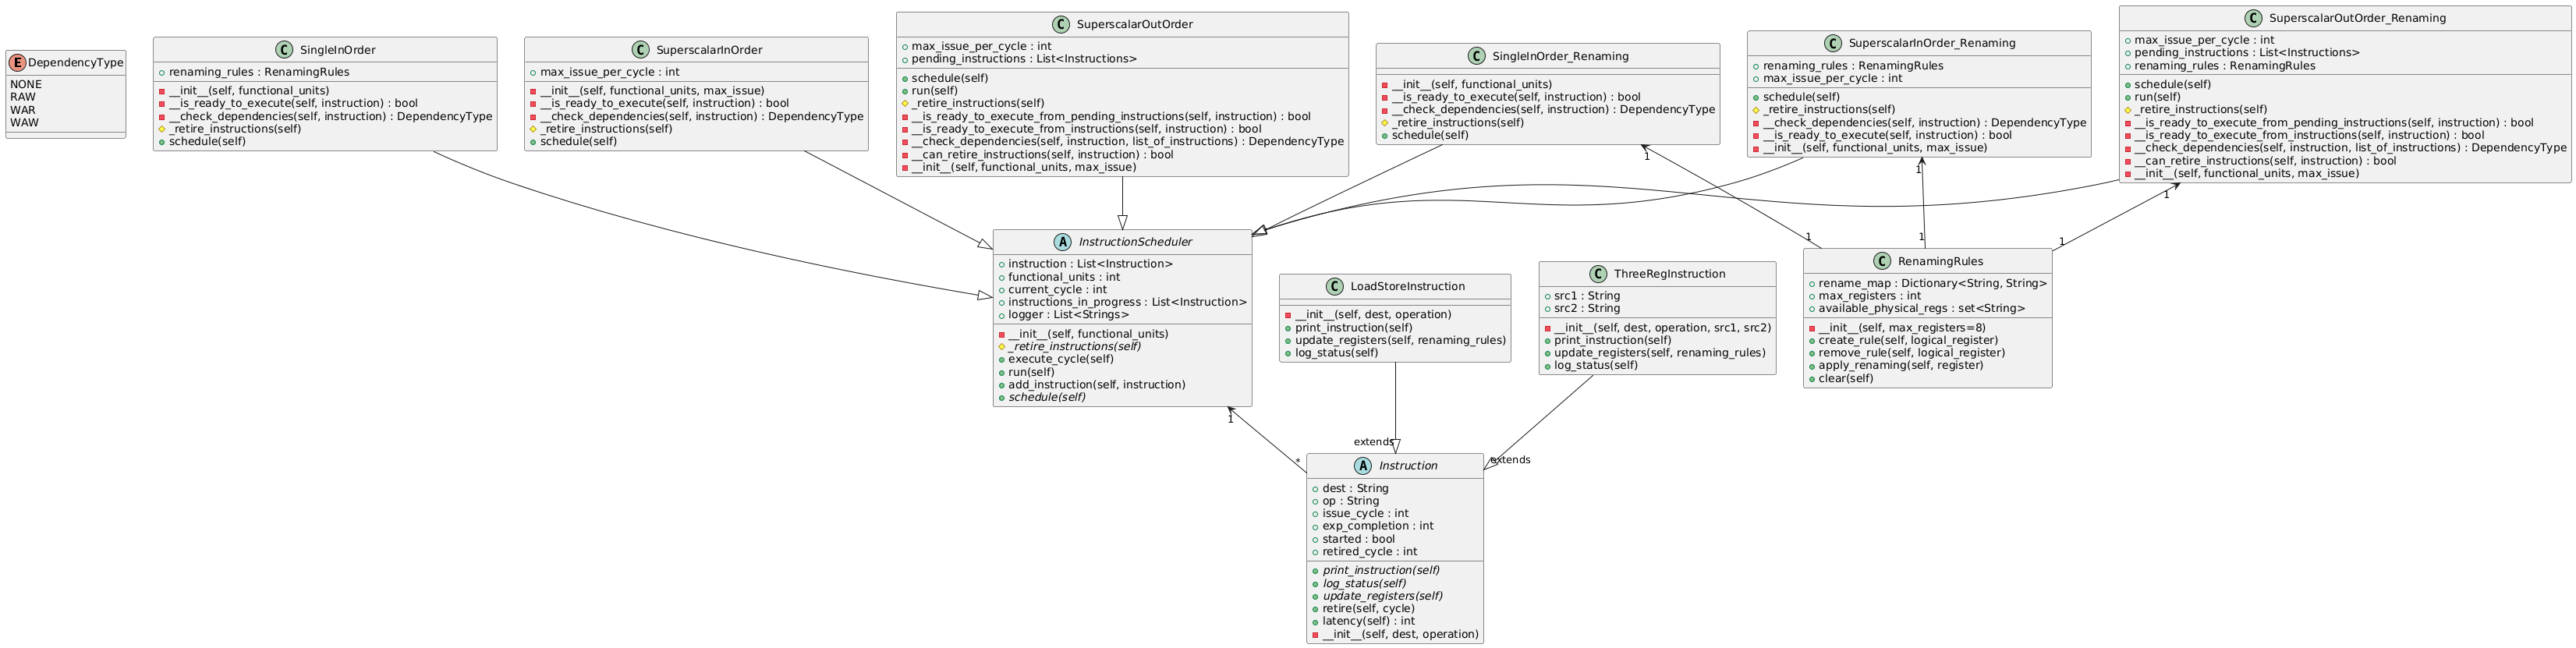
\includegraphics[width=1\textwidth]{ClassDiagram.png}  
    \caption{Class Diagram of Design, developed using the Plant UML tools.}  
    \label{fig:ClassDiagram}
\end{figure}

The diagram in figure \ref{fig:ClassDiagram} encapsulates the logic that helped develop this simulation. In the following subsections, I will be explaining each class with code snippets and implementation to justify each of the components. Before, delving into the overall classes let's discuss the format of the assembly instructions. 

\subsection{Assembly Format}
The assembly format contains various properties that were expected from the simulation, and some that I believed were proper. The properties that made up the assembly format can be explained with the following:

\begin{itemize}
    \item There are 8 fixed registers (R0 to R7) used in the assembly code
    \item There are only 5 instruction operations: +, -, *, LOAD, and STORE
    \item The format of the instructions are as follow: R1 = LOAD, R2 = STORE, R0 = R1 + R7, R1 = R2 * R3, etc\ldots
    \item +, - instructions take 1 cycle to complete
    \item * take 2 cycles to complete 
    \item LOAD, STORE take 3 cycles to complete
\end{itemize}

This assembly format ended up being used to develop the tests used to demonstrate proper functionality when simulating. The classes in charge of containing the instructions that derive from the assembly are the ones that compose the instruction hierarchy.

\subsection{Instruction Hierarchy}
The Instruction Hierarchy is used to encompass methods and data that provide access to the instructions as individual components when simulating, containing properties such as: source registers, destination registers, etc\ldots The parent class of this hierarchy is the \lstinline|Instruction| abstract class which contained the following properties:

\begin{itemize}
    \item \lstinline|dest|: this property looked to contain the destination register of an instruction. Allowing easy access to this information when required by the instruction schedulers.
    \item \lstinline|op|: this one contained the type of operation that the current instance is supposed to hold, determining the latency for further properties.
    \item \lstinline|issue_cycle|: this integer contained the processor cycle in which the instance of the instruction was issued.
    \item \lstinline|exp_completion|: this property contained the expected completion cycle for an instruction, stating after which point the instruction could be retired. 
    \item \lstinline|started|: this is a boolean that was raised when the instruction was issued, implying that I have (in a sense) been scheduled. 
    \item \lstinline|retired_cycle|: this property contained the actual cycle in which the instruction got retired by the processor configuration.
\end{itemize}

These properties were present in all types of instructions defined in the assembly format, the only work around done was that for `STORE' instructions filled the `destination register' with its source register. Thus, leading to certain checks when handling dependencies.

The methods in this class, were used to extract information from the instructions themselves, so that the code would be less repeated. 

\begin{itemize}
    \item \lstinline|print_instruction(self)|: abstract method in charge of printing instructions. This is used to print out each instruction in the command line.
    \item \lstinline|log_status(self)|: abstract method in charge of logging the status of the instruction at given points of the scheduling. This method logs the issue cycle and the retire cycle when called. Used for debugging and printing.
    \item \lstinline|update_registers(self, renaming_rules)|: abstract method in charge of updating the source registers that compose an instruction based on the renaming rules, basically applying renaming rules.
    \item \lstinline|retire(self, cycle)|: method in charge of retiring an instruction when called. Used when an instruction has been completely scheduled, exited the pipeline.
    \item \lstinline|latency(self)|: method in charge of retrieving the latency of any instruction, used for calculating some of the properties.
\end{itemize}

This abstract class does not represent instructions as a whole. Instead they represent a base for the concrete types of instructions that inherit from them. The concrete classes that inherit from \lstinline|Instruction| are \lstinline|LoadStoreInstruction| and \lstinline|ThreeRegInstruction|.
\subsubsection{Three Register Instructions}
The \lstinline|ThreeRegInstruction| class contains two more properties: \lstinline|src1| and \lstinline|src2|; and defines the abstract methods with their desired behavior. These properties combined with the properties from the parent class \lstinline|Instruction| allow an instance to represent a Three Register Instruction such as: R1 = R2 + R3.

\subsubsection{Load and Store Instructions}
The \lstinline|LoadStoreInstruction| only defines the abstract methods from \lstinline|Instruction| allowing an instance of itself to represent a Load or a Store Instruction such as: R1 = STORE. Now that we understand the representation of instructions we may begin looking at how register renaming rules were implemented. 

\subsection{Register Renaming Rules}
Register renaming rules were implemented with a class that was a part of any processor configuration that contained the technique. The class was named \lstinline|RenamingRules| and it contained properties and methods in charge of handling, applying and removing renaming rules as the scheduling of a set of instructions took place. The properties it contained were as follows:

\begin{itemize}
    \item \lstinline|rename_map|: this essentially a dictionary that relates a register from assembly (logical register) to a hidden register (physical register), like a rule relating the two. 
    \item \lstinline|max_registers|: the maximum number of registers, this represents the physical registers that were used when applying the register renaming technique. Represented by registers such as: S0, S7, etc.
    \item \lstinline|available_physical_registers|: represent the remaning number of registers available for renaming based on the number of renaming rules currently in place. 
\end{itemize}

The properties in this class are used to represent renaming rules in the program, yet to create new rules and delete invalid rules, I created two methods in charge of this. Those methods are:

\begin{itemize}
    \item \lstinline|create_rule(self, logical_register)|: this method creates a rule for the logical register it receives (e.g: \lstinline|R0 => S1|). The code in charge of doing this is fairly simple. 
\begin{lstlisting}[language=Python]
    def create_rule(self, logical_register):
        if logical_register not in self.rename_map:
            if not self.available_physical_regs:
                return False 
            physical_register = self.available_physical_regs.pop() 
            self.rename_map[logical_register] = physical_register
            return True
        return False
\end{lstlisting}
    This snippet of the program creates a mapping between one of the available hidden registers and the register it received as input. 
    \item \lstinline|remove_rule(self, logical_register)|: this method is in charge of removing rules for a certain logical register, it looks to invalidate existing renaming rules. The function is as follows:
\begin{lstlisting}[language=Python]
        if logical_register in self.rename_map:
            physical_register = self.rename_map.pop(logical_register)
            self.available_physical_regs.add(physical_register) 
            return True
        return False
\end{lstlisting}
    Essentially, it removes the mapping between the logical register and the hidden register; and returns the hidden register to an available state. 
\end{itemize}

The use of the properties and methods in \lstinline|RenamingRules| in coordination with the processor scheduling configuration leads the technique of register renaming to be properly simulated in this program. Now, let's delve into the instruction schedulers.

\subsection{Instruction Scheduler Hierarchy}
The Instruction Scheduler Hierarchy is the family of classes that contain the main logic of the scheduling simulation. The parent class of this hierarchy is \lstinline|InstructionScheduler| class which contains a layout of properties and methods to develop each configuration. All other classes that persist above it are the concrete classes.

This section looks to encompass the most important concepts that simulate the desired behavior of each configuration. To understand this we won't look at individual classes but more at what overlapping techniques, properties and functions look like, and look to explain what each part looks to provide to a scheduler class.  This is done, because each configuration (set of capabilities) is a selection of these components. 

Let's begin by looking at the list of all the properties that the classes in this hierarchy contain, explaining what they provide and which classes contain them.

\begin{itemize}
    \item \lstinline|instructions|: a list of instructions that need to be scheduled by the current configuration. \textbf{All configurations} contain this. 
    \item \lstinline|functional_units|: the number of parallel functional units a process configuration has. \textbf{All configurations} contain this.
    \item \lstinline|current_cycle|: contains the current cycle being executed by the processor. \textbf{All configurations} contain this.
    \item \lstinline|instructions_in_progress|: contains the list of instructions that are in functional units, currently being executed. \textbf{All configurations} contain this.
    \item \lstinline|logger|: contains a list of strings that represent debug messages and statements of actions that are taking place while scheduling. \textbf{All configurations} contain this, and it represents a list of outputs.
    \item \lstinline|max_issue_per_cycle|: the number of issue slots per cycle for a certain configuration. Only \textbf{Superscalar configurations} contain this property, because it represents it indicates how many instructions should be attempted per executed cycle.
    \item \lstinline|pending_instructions|: a list of instructions that have been overlooked/skipped by the processor configuration. This list is only present in \textbf{configurations with Out of Order execution}.
    \item \lstinline|renaming_rules|: contains an instance of the \lstinline|RenamingRules| class to create, delete and map renaming rules. This instance is only present in configurations with \textbf{Register Renaming technique}. 
\end{itemize}

The properties stated aforementioned are combined in various ways to provide the information necessary to achieve the desired behavior of the instruction scheduler configurations stated in the beginning of this report document.

The methods in this hierarchy are mostly different with a certain set of features that are the same for all. These features, come from overlapping behaviors and can be encapsulated in the following bulletpoints:

\begin{itemize}
    \item \lstinline{add_instruction(self, instruction)}: this method is in charge of adding an instruction to \lstinline|instructions| of each instance. It is used to input the instruction set from the file.
    \item \lstinline{execute_cycle(self)}: this method contains the logic of executing a cycle; increment cycle, schedule instructions, and retire instructions. It does so by performing these commands:
    \begin{lstlisting}[language=Python]
    def execute_cycle(self):
        self.current_cycle += 1
        self.schedule()
        self._retire_instructions()
    \end{lstlisting}
    \item \lstinline|_schedule_instruction(self, instr)|: this method is in charge of scheduling an instruction whenever called. This requires the following logic: 
    \begin{lstlisting}[language=Python]
    def _schedule_instruction(self, instr : Instruction):
        instr.issue_cycle = self.current_cycle
        instr.exp_completion = self.current_cycle + instr.latency()
        instr.started = True 
        self.instructions_in_progress.append(instr)
    \end{lstlisting}
    Were some of the instruction's properties get modified, and the instruction being scheduled is added to the list of instructions in progress. 
    \item \lstinline|run(self)|: this method is in charge of repeatedly running cycles until all instructions have been processed. For most configurations it has this format:
    \begin{lstlisting}
    def run(self):
        while self.instructions or self.instructions_in_progress:
            self.execute_cycle()
    \end{lstlisting}
\end{itemize}

The three items that were just described are consistent throughout all, but they don't contain the whole logic behind the instruction scheduling and instruction retiring. The core logic of this simulation is found in the \lstinline|schedule| and \lstinline|_retire_instructions| methods. As a quick description each configuration type (for both, with or without register renaming) has a different format for scheduling and retiring.

\subsubsection{Single-issue Instruction Scheduler Configurations}
Single-issue Instruction Scheduler configurations use in-order execution and retirement, this implies that both versions of this format use the same logic for instruction scheduling. The method in charge of this is the following:

\begin{lstlisting}[language=Python]
def schedule(self):
    if len(self.instructions_in_progress) < self.functional_units and self-
    .instructions:
        instr = self.instructions[0]
        if self.__is_ready_to_execute(instr):
            self._schedule_instruction(instr)
            self.instructions.remove(instr) 
\end{lstlisting}

This version of the schedule logic is in charge of looking at the instruction list as a queue, were every cycle you can only check if you can schedule the oldest instruction. This method checks if there is space to schedule an instruction, and if there are remaining instructions to schedule. It only schedules instruction that are ready to execute. 

Being ready to execute implies checking data dependencies, and looking to resolve them when there is register renaming. Thus, implying that the difference between the two versions of Single-issue Instruction Scheduler's rellies on the checking if an instruction is ready to execute.

In the original version (no register renaming) the methods used for checking readiness of an instruction before scheduling is as follows:

\begin{lstlisting}[language=Python]
def __is_ready_to_execute(self, instruction):
    return self.__check_dependencies(instruction) == DependencyType.NONE
    
def __check_dependencies(self, instruction):
    for instr in self.instructions_in_progress:
        if (isinstance(instruction, ThreeRegInstruction)) 
        and instr.dest in [instruction.src1, instruction.src2]:
            return DependencyType.RAW
        if instruction.op == "STORE" and instr.dest == instruction.dest:
            return DependencyType.RAW
        if isinstance(instr, ThreeRegInstruction) 
        and instruction.dest in [instr.src1, instr.src2]:
            return DependencyType.WAW
        if instruction.dest == instr.dest:
            return DependencyType.WAW
    return DependencyType.NONE
\end{lstlisting}

The methods stated above contain the logic for checking if there is a data dependency, and only allow instructions that have no data dependencies to be executed. The return values seen in the method \lstinline|__check_dependencies(self, instruction)| are an enum used to describe the data dependency types differentiate between them.

The version with register renaming of this configurations has the same logical checks but with the difference that in the method \lstinline| __is_ready_to_execute(self, instruction)| we first update the source registers and check if the destination register implies the invalidation of a renaming rule, before checking for data dependencies. Also, any write-after data dependencies are solved with the creation of register renaming rules.

Lastly, in-order instruction retirement is performed in the same manner for both versions of this configuration. Were we look to try and retire in the order of First Come, First Retired like a queue. This logic is defined in the following method:

\begin{lstlisting}[language=Python]
def _retire_instructions(self): 
    for instr in self.instructions_in_progress[:]:
        if self.current_cycle >= instr.exp_completion:
            instr.retire(self.current_cycle)
            self.logger.append(f"{instr.log_status()}")
            self.instructions_in_progress.remove(instr)
        else:
            break
\end{lstlisting}

This method looks at the list of instructions in progress and tries to retire the oldest instruction first, if it can't it waits until the cycle in which the oldest instruction can be retired otherwise it just continues doing this with the second to oldest instruction.

\subsubsection{Superscalar Instruction Scheduler Configurations}
In this section we will be discussing the logic behind all versions of superscalar instruction scheduler configurations. As a quick description, these configurations attempt to issue multiple instructions at the same time. There are two main versions: in-order execution and retirement (simplest) and out of order execution and retirement (complex). Let's begin by discussing the first.

\paragraph{In-Order Execution and Retirement}
Interestingly enough, both In-order Superscalar Instruction Scheduler versions only have one modification; that achieves the desired behavior; from their Single Instruction Scheduler counterparts. Which is iterating various times in the scheduling of an instruction based on the issue slots available. This is achieved by only modifying the schedule method while maintaining the rest of the logic the same. 

\begin{lstlisting}[language=Python]
def schedule(self):
    attempted_issues = 0
    for instruction in self.instructions[:]:
        if len(self.instructions_in_progress) < self.functional_units 
        and attempted_issues < self.max_issue_per_cycle:
            attempted_issues += 1
            if self.__is_ready_to_execute(instruction):
                self._schedule_instruction(instruction)
                self.instructions.remove(instruction)
            else:
                break
\end{lstlisting}

This method allows the behavior of a superscalar in-order instruction scheduler to be achieved. I decided to not explain the rest since we already have the explanation in the section before.

\paragraph{Out of Order Execution and Retirement}
This family of configurations bring a lot of complexity to the equation. Since, these classes of configurations require instructions to be issued from both the list of pending instructions and the list of instructions. Thus, requiring two different types of checks. Before analysing the checks, we may begin by looking at how out of order execution is achieved.

\begin{lstlisting}[language=Python]
def schedule(self):
    attempted_issues = 0
    for pending in self.pending_instructions[:]:
        if len(self.instructions_in_progress) < self.functional_units:
            if self.__is_ready_to_execute_from_pending_instructions(pending):
                self._schedule_instruction(pending)
                self.pending_instructions.remove(pending)

    for instruction in self.instructions[:]:
        if len(self.instructions_in_progress) < self.functional_units 
        and attempted_issues < self.max_issue_per_cycle:
            attempted_issues += 1
            if self.__is_ready_to_execute_from_instructions(instruction):
                self._schedule_instruction(instruction)
                self.instructions.remove(instruction)
            else:
                self.pending_instructions.append(instruction)
                self.instructions.remove(instruction)
\end{lstlisting}

The reasoning behind this method is that we attempt first instructions that have been overlooked (pending instructions), trying to see if the dependencies have already been resolved and we try to schedule them. And once we have tried all possible pending instructions we move on to issue as many new instructions as allowed by the number of issue slots; if new instructions can't be scheduled we overlook them. This process allows instructions to be executed out of order as long as no dependencies exist.

The process of checking dependencies is similar to the ones mentioned before, with the exception that when we schedule instructions from the list of instructions we must check that there are no dependencies with all pending and in progress instructions. Meanwhile, when we process instructions from the list of pending instructions we must check that there are no dependencies with in-progress instructions or with instructions that were overlooked before the current one being processed. 

The version of this configuration with \textbf{register renaming} does the same process of trying to resolve write-after data dependencies with both pending and in-progress instructions, considering the past constraint. Yet, source registers can only be updated by renaming rules when the instruction being processed comes from the original list of instructions.

Out of order retiring was achieved by attempting to retire any in-progress instructions if they had already been completed and writing to their destination registers wouldn't imply any discrepencies between the desired logic of the assembly instructions. The methods that help implement this logic are:

\begin{lstlisting}[language=Python]
def _retire_instructions(self):
    i = 0 
    while i < len(self.instructions_in_progress):
        instr = self.instructions_in_progress[i]
        if self.current_cycle >= instr.exp_completion 
        and self.__can_retire_instructions(instr):
            instr.retire(self.current_cycle)
            self.logger.append(f"{instr.log_status()}")
            self.instructions_in_progress.pop(i)
        else:
            i += 1
    
def __can_retire_instructions(self, instruction):
    for instr in self.instructions_in_progress:
        if instr.issue_cycle < instruction.issue_cycle:
            if isinstance(instr, ThreeRegInstruction) 
            and instruction.dest in [instr.src1, instr.src2]:
                return False
            if instr.dest == instruction.dest
            and instruction.op != 'STORE':
                return False
    return True
\end{lstlisting}

These methods are the implemented logic that check if an instruction may be retired, and completing the process of scheduling instructions by completely retiring them. This is done in this manner to prevent instructions to be retired while not maintaining the proper logic of the program.

And lastly, for all instructions to be processed properly the \lstinline|run| method had to be overwritten for it to also consider the list of pending instructions:
\begin{lstlisting}[language=Python]
 def run(self):
    while self.instructions or self.instructions_in_progress 
    or self.pending_instructions:
        self.execute_cycle()
\end{lstlisting}

With all these being said, we have discussed the entire implementation and design of the program I developed for this project. It is important to understand that this explanation contains the main concepts that lead to the desired behavior but fails to explain all methods and properties with utmost detail. Yet, the actual behavior applied is mentioned for all. If you'd want a better understanding it is better to look at the source files while reading the Methodology section to further familiarize with the implementation. All snippets of code in this section, are uncommented versions.

\section{Validation \& Verification}
The design demonstrates the logic utilized, but we need to visualize that the implementation discussed in the past section has the desired behavior. To do so, we will be comparing the results of my simulation against those seen in class as to demonstrate whether the simulation is correct. 

\begin{figure}[H]
    \begin{lstlisting}
                                R3 = R0 * R1
                                R4 = R0 + R2
                                R5 = R0 + R1
                                R6 = R1 + R4
                                R7 = R1 * R2
                                R1 = R0 - R2
                                R3 = R3 * R1
                                R1 = R4 + R4  
    \end{lstlisting}
    \caption{This is the set of assembly instruction's analyzed during the Case Study's in class.}
    \label{fig:CaseStudyAssembly}
\end{figure}

We will first write the configuration and demonstrate the results for the class results in the left hand side and the screenshot of the results in my program.
\newpage
\begin{enumerate}
    \item Superscalar In-order Instruction Scheduler with 2 Issue Slots and No Register Renaming. This configuration is the one we studied for Case Study 1.
    \begin{figure}[H]
        \centering{}
        \begin{minipage}[t]{0.45\textwidth}
            \centering
            \renewcommand{\arraystretch}{0.8} % Increases row height for readability
            \setlength{\tabcolsep}{3pt} % Adjusts padding between columns
            \begin{tabular}{|c|p{3.4cm}|c|}
                \hline
                \textbf{Cycle} & \textbf{Instructions Issued} & \textbf{Retired} \\ \hline
                1 & 1. R3 = R0 * R1 & \\ 
                  & 2. R4 = R0 + R2 & \\ \hline
                2 & 3. R5 = R0 + R1 & \\ 
                  & \sout{4. R6 = R1 + R4} & \\ \hline
                3 &                 & \\ \hline
                 &                 & 1 \\ 
                4 &                 & 2 \\ 
                 &                 & 3 \\ \hline
                5 & 4. R6 = R1 + R4 & \\
                  & 5. R7 = R1 * R2 & \\ \hline 
                6 & \sout{6. R1 = R0 - R2} & \\ \hline
                7 & & 4 \\ \hline 
                8 & & 5 \\ \hline 
                9 & 6. R1 = R0 - R2 & \\ \hline
                  & \sout{7. R3 = R3 * R1} & \\ \hline
                10 & & \\ \hline 
                11 & & 6 \\ \hline 
                12 & 7. R3 = R3 * R1 & \\ \hline 
                & \sout{8. R1 = R4 + R4} & \\ \hline
                13 & & \\ \hline
                14 & & \\ \hline 
                15 & & 7 \\ \hline 
                16 & 8. R1 = R4 + R4 & \\ \hline 
                17 & & \\ \hline 
                18 & & 8 \\ \hline 
            \end{tabular}
        \end{minipage}
        \begin{minipage}[t]{0.45\textwidth}
            \renewcommand{\arraystretch}{1} % Increases row height for readability
            \setlength{\tabcolsep}{3pt} % Adjusts padding between columns
            \begin{tabular}{|p{3.4cm}|c|c|}
                \hline
                \textbf{Instruction} & \textbf{Issued} & \textbf{Retired} \\ \hline
                1. R3 = R0 * R1 & 1 & 4 \\ \hline 
                2. R4 = R0 + R2 & 1 & 4 \\ \hline 
                3. R5 = R0 + R1 & 2 & 4 \\ \hline 
                4. R6 = R1 + R4 & 5 & 7 \\ \hline 
                5. R7 = R1 * R2 & 5 & 7 \\ \hline
                6. R1 = R0 - R2 & 9 & 11 \\ \hline
                7. R3 = R3 * R1 & 12 & 15 \\ \hline 
                8. R1 = R4 + R4 & 16 & 18 \\ \hline 
            \end{tabular}
            \newline 
            \newline        
            The results from my simulation; although formatted differently, demonstrate the exact same behavior as the results from the case study. This proves that the simulation, at least for Superscalar In-order Instruction Schedulers with no renaming, is proper.
        \end{minipage}
        \caption{Comparison of simulation results for the in-class case study 1 (left) and custom configuration (right).}
    \end{figure}
    \newpage
    \item Superscalar In-order Instruction Scheduler with 2 Issue Slots and Register Renaming. This is the configuration we studied for Case Study 2 in class. 
    \begin{figure}[H]
        \centering
        \begin{minipage}[t]{0.45\textwidth}
            \centering
            \renewcommand{\arraystretch}{0.9} % Adjusts row height
            \setlength{\tabcolsep}{3pt} % Adjusts column padding
            \begin{tabular}{|c|p{3.4cm}|c|}
                \hline
                \textbf{Cycle} & \textbf{Instructions Issued} & \textbf{Retired} \\ \hline
                1 & 1. R3 = R0 * R1 & \\ 
                  & 2. R4 = R0 + R2 & \\ \hline
                2 & 3. R5 = R0 + R1 & \\ 
                  & \sout{4. R6 = R1 + R4} & \\ \hline
                3 &                 & \\ \hline
                  &                 & 1 \\ 
                4 &                 & 2 \\ 
                  &                 & 3 \\ \hline
                5 & 4. R6 = R1 + R4 & \\
                  & 5. R7 = R1 * R2 & \\ \hline 
                6 & 6. R1 = R0 - R2 & \\ 
                  & \sout{7. R3 = R3 * R1} & \\ \hline 
                7 &                 & 4 \\ \hline 
                8 &                 & 5 \\ \hline 
                  &                 & 6 \\ \hline 
                9 & 7. R3 = R3 * R1 & \\ 
                  & 8. R1 = R4 + R4 & \\ \hline 
               10 &                 & \\ \hline 
               11 &                 & \\ \hline 
               12 &                 & 7 \\ 
                  &                 & 8 \\ \hline 
            \end{tabular}
        \end{minipage}
        \begin{minipage}[t]{0.45\textwidth}
            \centering
            \renewcommand{\arraystretch}{1.2} % Adjusts row height
            \setlength{\tabcolsep}{3pt} % Adjusts column padding
            \begin{tabular}{|p{3.4cm}|c|c|}
                \hline
                \textbf{Instruction} & \textbf{Issued} & \textbf{Retired} \\ \hline
                1. R3 = R0 * R1 & 1 & 4 \\ \hline 
                2. R4 = R0 + R2 & 1 & 4 \\ \hline 
                3. R5 = R0 + R1 & 2 & 4 \\ \hline 
                4. R6 = R1 + R4 & 5 & 7 \\ \hline 
                5. R7 = R1 * R2 & 5 & 8 \\ \hline
                6. R1 = R0 - R2 & 6 & 8 \\ \hline
                7. R3 = R3 * R1 & 9 & 12 \\ \hline 
                8. R1 = R4 + R4 & 9 & 12 \\ \hline 
            \end{tabular}
            \vspace{1em} % Adds vertical space
            \raggedright

            The results of both my simulation and the in-class case study are consistent, proving that the Superscalar In-order Instruction Scheduler with Renaming provides the desired behavior.
        \end{minipage}
        \caption{Comparison of simulation results for the in-class case study 2 (left) and custom configuration (right).}
    \end{figure}
    \newpage
    \item Superscalar Out-of-order Instruction Scheduler with 2 Issue Slots and Register Renaming. This is the configuration we studied for Case Study 4 in class. 
    \begin{figure}[H]
        \centering
        \begin{minipage}[t]{0.45\textwidth}
            \centering
            \renewcommand{\arraystretch}{0.9} % Adjusts row height
            \setlength{\tabcolsep}{3pt} % Adjusts column padding
            \begin{tabular}{|c|p{3.4cm}|c|}
                \hline
                \textbf{Cycle} & \textbf{Instructions Issued} & \textbf{Retired} \\ \hline
                1 & 1. R3 = R0 * R1 & \\ 
                  & 2. R4 = R0 + R2 & \\ \hline
                2 & 3. R5 = R0 + R1 & \\ 
                  & \sout{4. R6 = R1 + R4} & \\ \hline
                3 & 5. R7 = R1 * R2 & \\ 
                  & 6. S1 = R0 - R2 & \\
                  & & 2 \\ \hline 
                4 & 4. R6 = R1 + R4 & \\ 
                  & \sout{7. R3 = R3 * S1} & \\
                  & 8. S2 = R4 + R4 & \\
                  & & 1 \\
                  & & 3 \\ \hline 
                5 & & 6 \\ \hline 
                6 & 7. R3 = R3 * S1 & \\
                & & 4 \\ 
                & & 5 \\ 
                & & 8 \\ \hline 
                7 & & \\ \hline 
                8 & & \\ \hline 
                9 & & 7 \\ \hline 
            \end{tabular}
        \end{minipage}
        \begin{minipage}[t]{0.45\textwidth}
            \centering
            \renewcommand{\arraystretch}{1.2} % Adjusts row height
            \setlength{\tabcolsep}{3pt} % Adjusts column padding
            \begin{tabular}{|p{3.4cm}|c|c|}
                \hline
                \textbf{Instruction} & \textbf{Issued} & \textbf{Retired} \\ \hline
                2. R4 = R0 + R2 & 1 & 3 \\ \hline 
                1. R3 = R0 * R1 & 1 & 4 \\ \hline 
                3. R5 = R0 + R1 & 2 & 4 \\ \hline 
                6. S4 = R0 - R2 & 3 & 5 \\ \hline 
                5. R7 = R1 * R2 & 3 & 6 \\ \hline 
                4. R6 = R1 + R4 & 4 & 6 \\ \hline 
                8. S3 = R4 + R4 & 4 & 6 \\ \hline 
                7. R3 = R3 * S4 & 6 & 9 \\ \hline 
            \end{tabular}
            \vspace{1em} % Adds vertical space
            \raggedright

            The results allthough formatted differently have the same behavior. Proving that also the Superscalar Out-of-order Instruction Scheduler with Renaming works properly. 
        \end{minipage}
        \caption{Comparison of simulation results for the in-class case study 2 (left) and custom configuration (right).}
    \end{figure}
\end{enumerate}

I believe that this set of examples are enough to validate and verify that the simulation does provide proper behavior. These tests were only developed to demonstrate that the simulation was fruitful, and that it does achieve the prerequisites of this project. 

\section{Tests}
With this we can begin to look at all configurations handling an individual test, that contains the correct latencies of: ``+'', ``-'' take 1 cycle, ``*'' take 2 cycles, and ``LOAD'' and ``STORE'' instructions take 3; and that contains all sort of data dependencies without the need of worrying if it works properly and only analysing the improvement each configuration was able to achieve in regards of instruction throughput.

The test that will be used to verify the relationship between the various techniques and instruction throughput is found in the ``test'' folder in the file ``instructions.asm''. This assembly ``program'' contains data dependencies between all types of instructions, testing the overall rigidness of this program and also demonstrating proper behavior. With this being said, let's look at the results for the following configurations (all with 4 functional units) both with and without register renaming.

\begin{enumerate}
    \item 1 issue slot, in-order 
    \item 1 issue slot, out-of-order issue and retirement 
    \item 2 issue slots, in-order 
    \item 2 issue slots, out-of-order issue and retirement 
    \item 3 issue slot, in-order 
    \item 3 issue slots, out-of-order issue and retirement 
\end{enumerate}

\section{Results}
This section contains screenshots of the results of simulating each of the aforementioned configurations. These results are only placed here to facilitate the visualization of outputs without the need to run the program for anyone reading this document or evaluating this project. Outputs will be placed for both register renaming (right) and no register renaming (left) version's of each configuration stated in the past section. 
\begin{enumerate}
    \item 1 issue slot, in-order results for 
    \begin{figure}[H]
        \centering 
        \begin{minipage}[t]{0.45\textwidth}
            \centering
            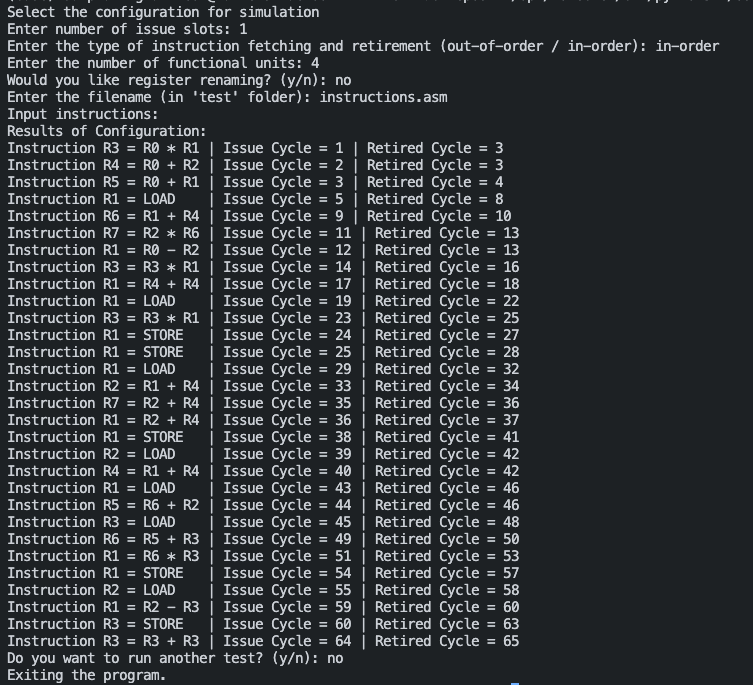
\includegraphics[width=\textwidth]{Images/Config1.png}
            \caption{1 issue slot, in-order configuration without register renaming.}
        \end{minipage}
        \hfill
        \begin{minipage}[t]{0.45\textwidth}
            \centering 
            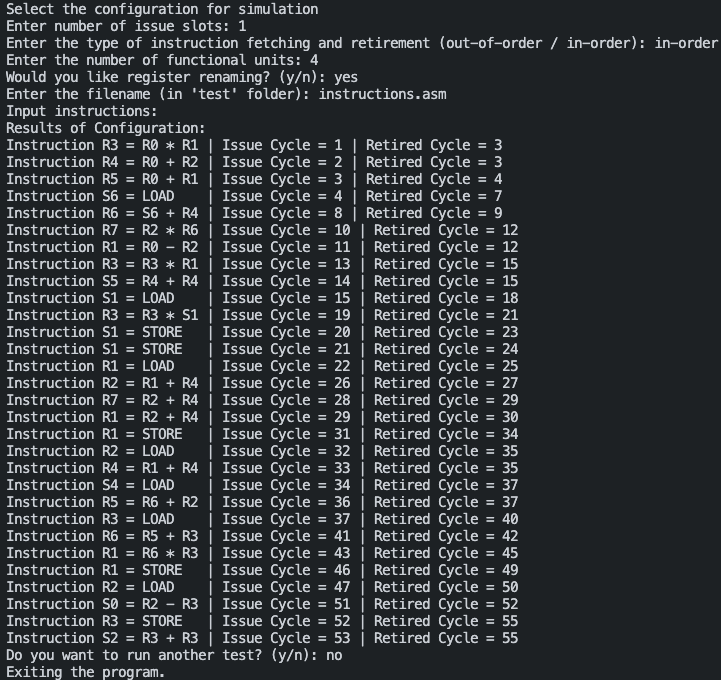
\includegraphics[width=\textwidth]{Images/Config1_Renaming.png}
            \caption{1 issue slot, in-order configuration with register renaming.}
        \end{minipage}
    \end{figure}

    \item 1 issue slot, out-of-order issue and retirement 
    \begin{figure}[H]
        \centering 
        \begin{minipage}[t]{0.45\textwidth}
            \centering
            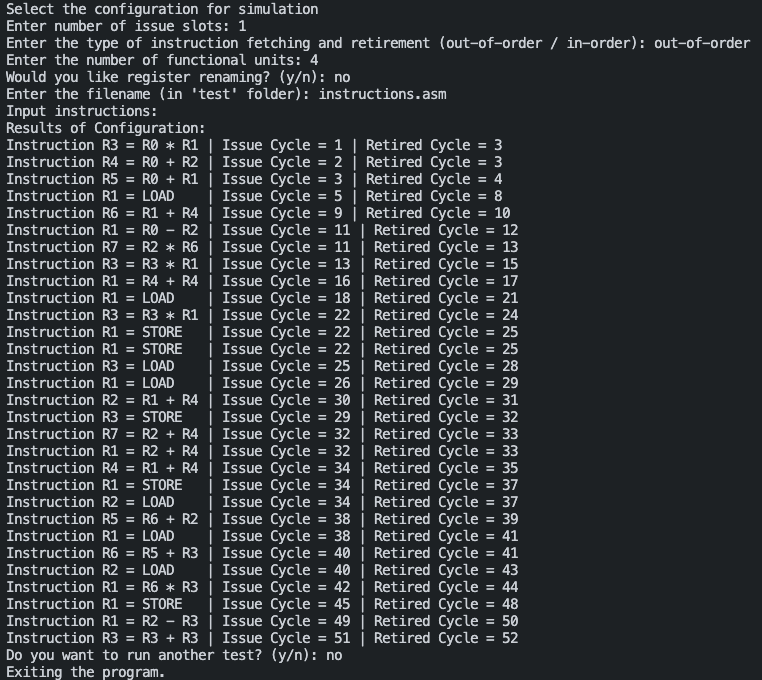
\includegraphics[width=\textwidth]{Images/Config2.png}
            \caption{1 issue slot, out-of-order issue and retirement configuration without register renaming.}
        \end{minipage}
        \hfill
        \begin{minipage}[t]{0.45\textwidth}
            \centering 
            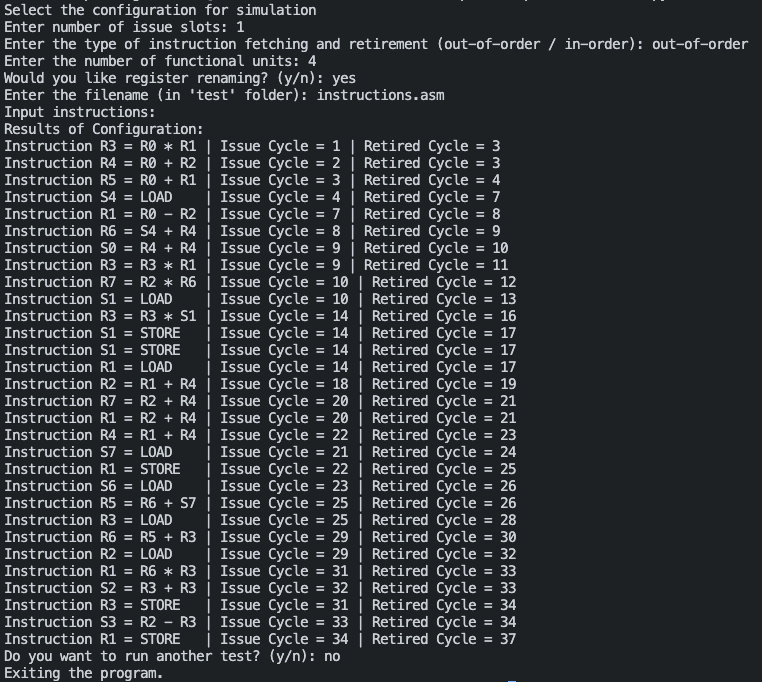
\includegraphics[width=\textwidth]{Images/Config2_Renaming.png}
            \caption{1 issue slot, out-of-order issue and retirement configuration with register renaming.}
        \end{minipage}
    \end{figure}

    \item 2 issue slots, in-order 
    \begin{figure}[H]
        \centering 
        \begin{minipage}[t]{0.45\textwidth}
            \centering
            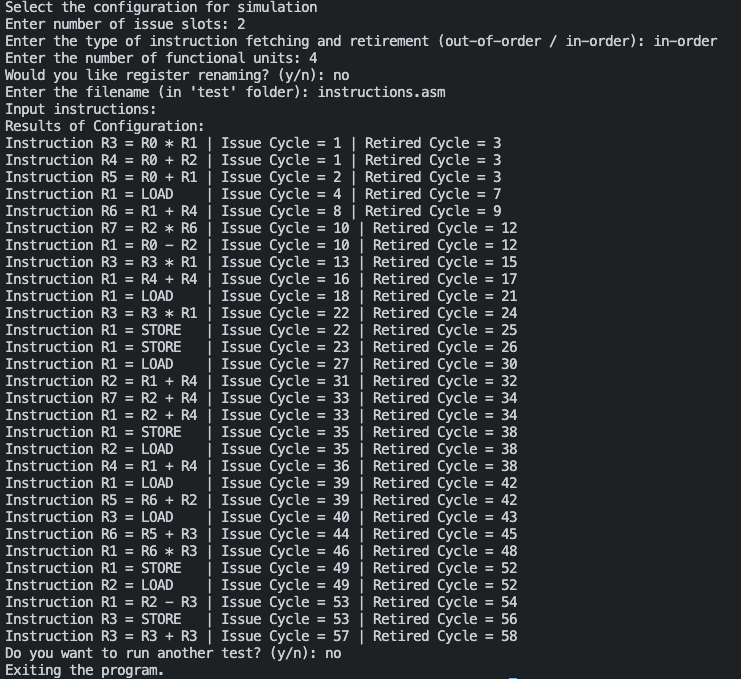
\includegraphics[width=\textwidth]{Images/Config3.png}
            \caption{2 issue slot, in-order configuration without register renaming.}
        \end{minipage}
        \hfill
        \begin{minipage}[t]{0.45\textwidth}
            \centering 
            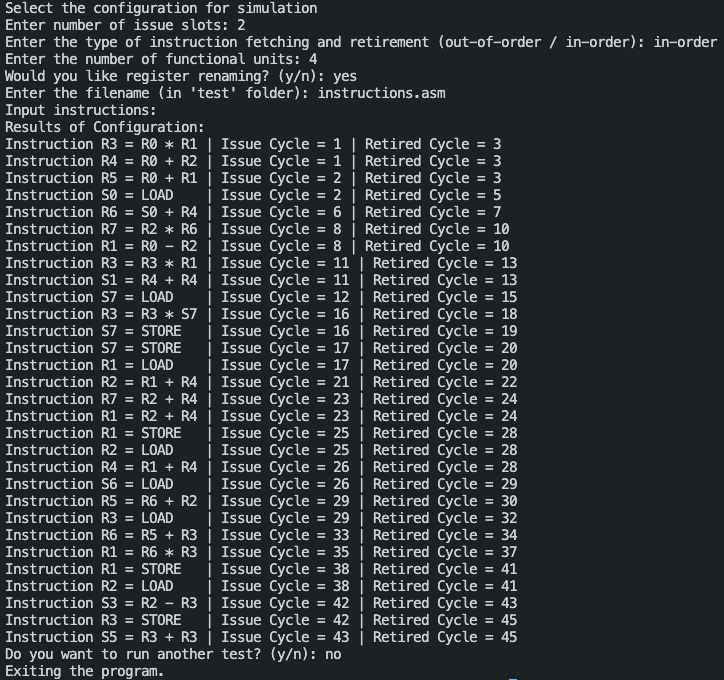
\includegraphics[width=\textwidth]{Images/Config3_Renaming.png}
            \caption{2 issue slot, in-order configuration with register renaming.}
        \end{minipage}
    \end{figure}

    \item 2 issue slots, out-of-order issue and retirement 
    \begin{figure}[H]
        \centering 
        \begin{minipage}[t]{0.45\textwidth}
            \centering
            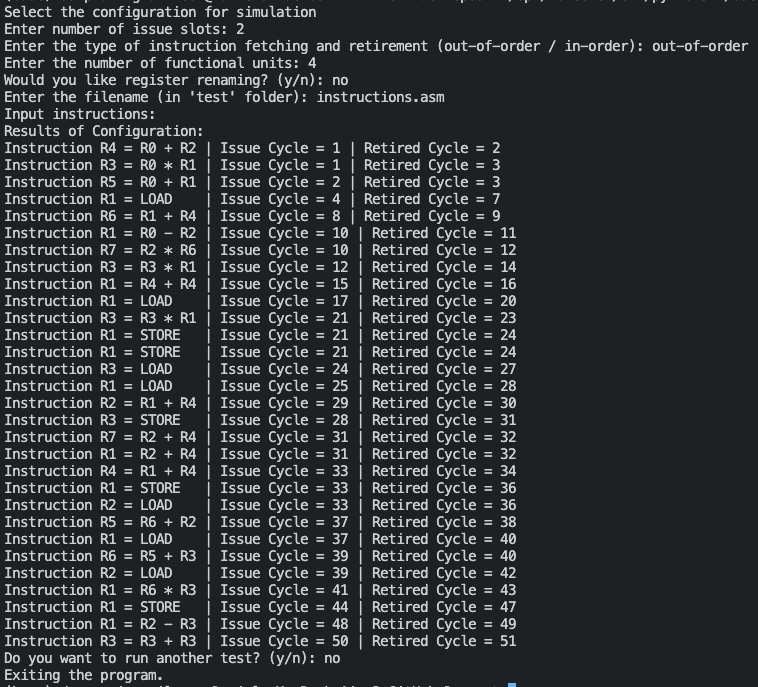
\includegraphics[width=\textwidth]{Images/Config4.png}
            \caption{2 issue slot, out-of-order issue and retirement without register renaming.}
        \end{minipage}
        \hfill
        \begin{minipage}[t]{0.45\textwidth}
            \centering 
            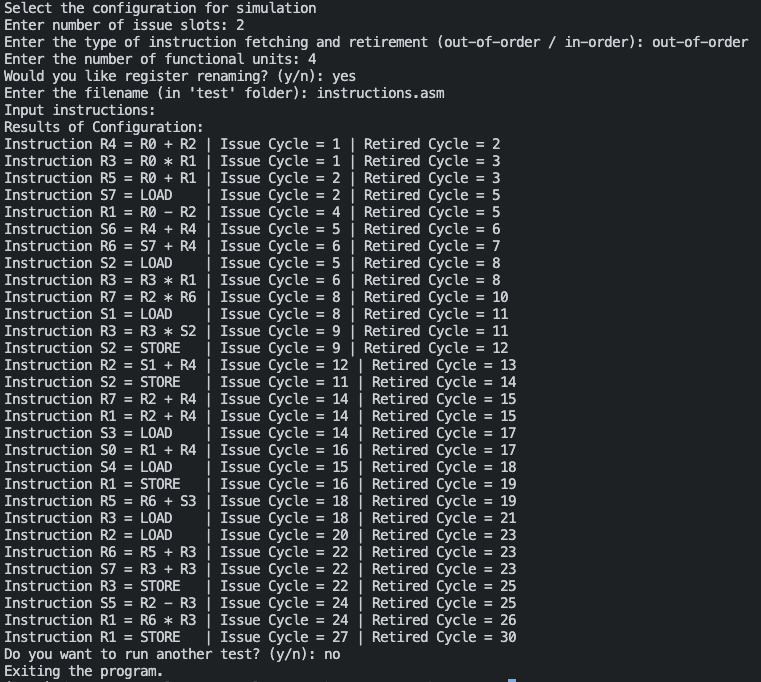
\includegraphics[width=\textwidth]{Images/Config4_Renaming.png}
            \caption{2 issue slot, out-of-order issue and retirement with register renaming.}
        \end{minipage}
    \end{figure}

    \item 3 issue slot, in-order
    \begin{figure}[H]
        \centering 
        \begin{minipage}[t]{0.45\textwidth}
            \centering
            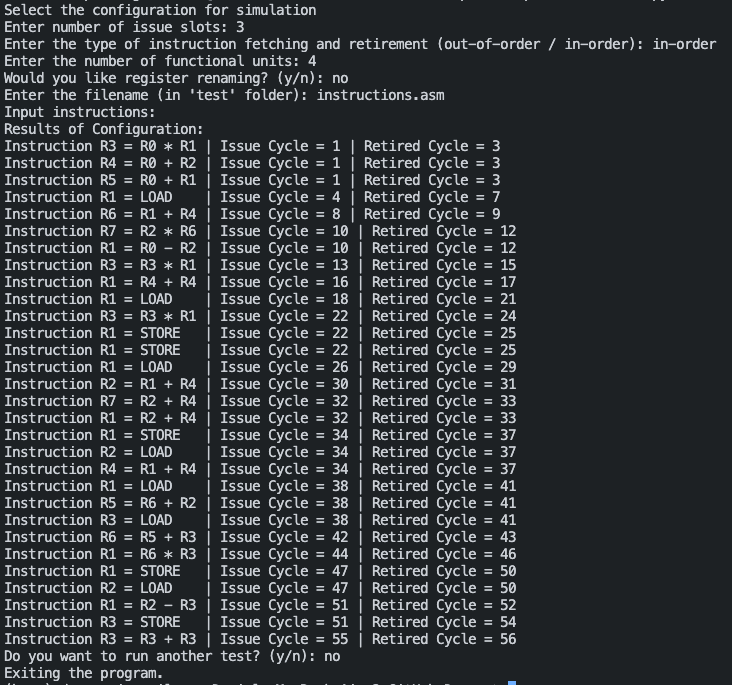
\includegraphics[width=\textwidth]{Images/Config5.png}
            \caption{3 issue slot, in-order configuration without register renaming.}
        \end{minipage}
        \hfill
        \begin{minipage}[t]{0.45\textwidth}
            \centering 
            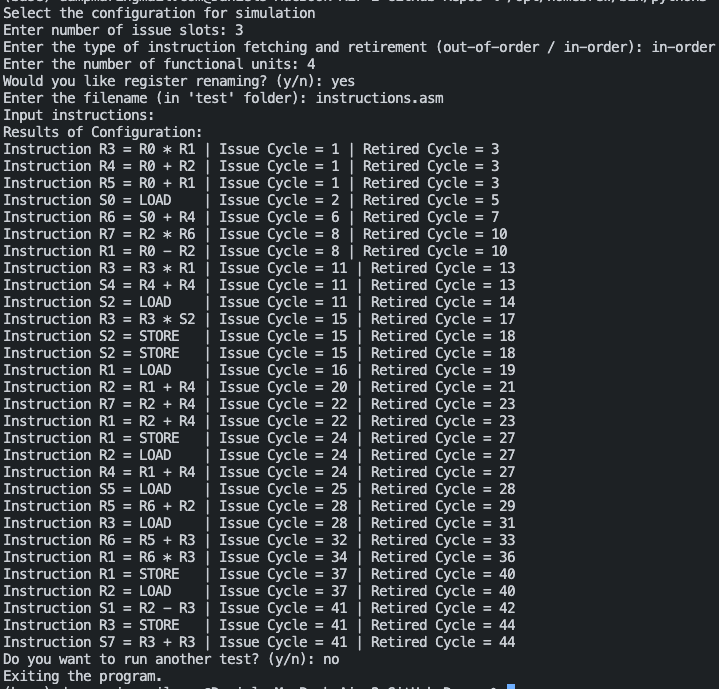
\includegraphics[width=\textwidth]{Images/Config5_Renaming.png}
            \caption{3 issue slot, in-order configuration with register renaming.}
        \end{minipage}
    \end{figure}

    \item 3 issue slots, out-of-order issue and retirement 
    \begin{figure}[H]
        \centering 
        \begin{minipage}[t]{0.45\textwidth}
            \centering
            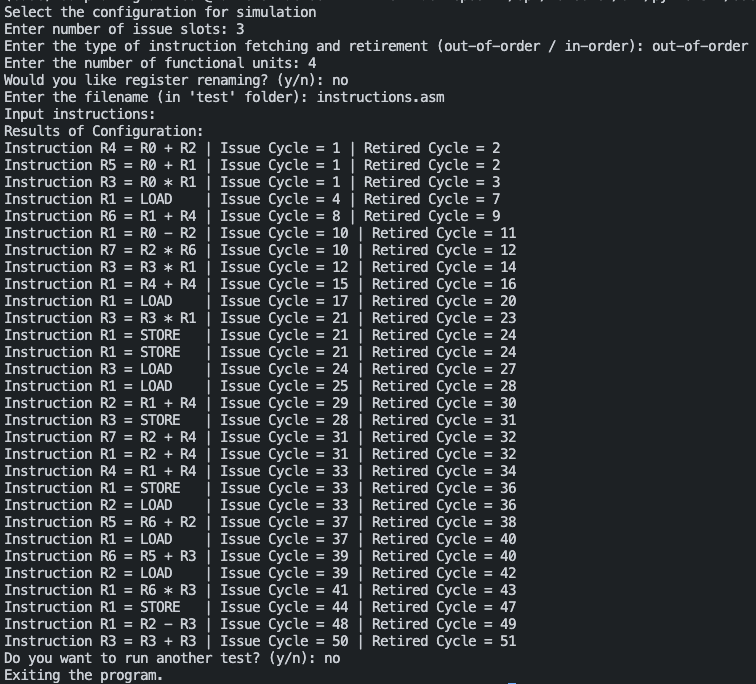
\includegraphics[width=\textwidth]{Images/Config6.png}
            \caption{3 issue slot, out-of-order issue and retirement without register renaming.}
        \end{minipage}
        \hfill
        \begin{minipage}[t]{0.45\textwidth}
            \centering 
            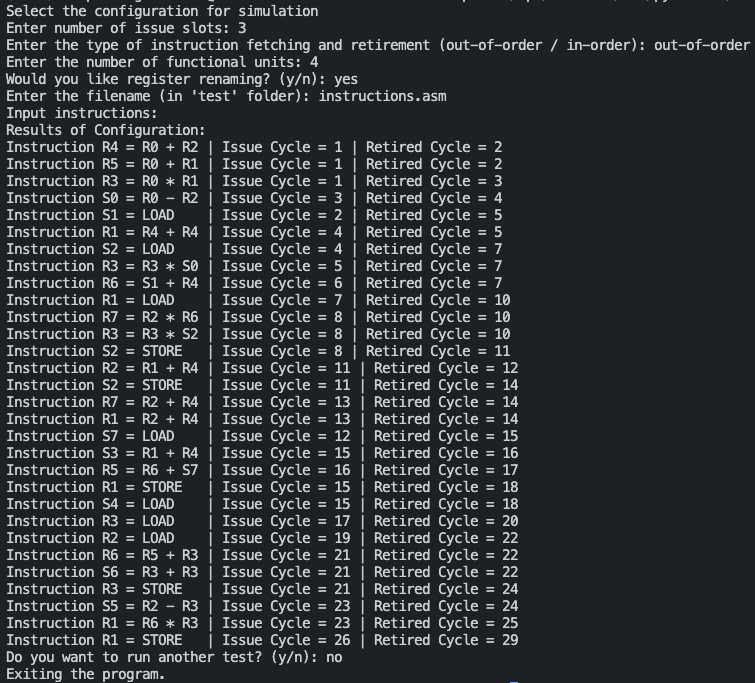
\includegraphics[width=\textwidth]{Images/Config6_Renaming.png}
            \caption{3 issue slot, out-of-order issue and retirement with register renaming.}
        \end{minipage}
    \end{figure}
\end{enumerate}

The results found in the past enumerate demonstrate the overall behavior for combinations of configurations. Were out-of-order superscalar instruction scheduler's with renaming out perform all other configurations. Various concepts discussed in class such as how the `sweetspot' for issue slots was of 2 and that out-of-order execution improves instruction throughput have been proven. Similar counterparts of 2 and 3 issue slots having nearly the same results; and counterparts with out-of-order execution and retirement have substantial boost in performance. 

It is important to state that proper handling between all types of data dependencies is demonstrated in all configurations as seen in the outputs found in Figure 6 through 17. 

\section{Discussion}

Instruction scheduling is a cornerstone of modern processor design, aimed at maximizing instruction throughput, minimizing stalls, and fully utilizing hardware resources/ Advanced techniques such as out-of-order execution and register renaming have been pivotal in optimizing instruction throughput, enabling processors to operate more efficiently. 

This project highlights the significant role of effective instruction scheduling in achieving more efficient processors. It demonstrates that the techniques studied in class, like: out-of-order execution and register renaming reduce idle cycles and resolve data dependencies dynamically, ensuring peak performance in computer systems; zooming into the critical importance of instruction scheduling in modern architectures. 
\end{document}